\documentclass[10pt,twocolumn]{article}
\usepackage[a4paper,margin=1.8cm,columnsep=0.6cm]{geometry}
\usepackage{amsmath,amssymb}
\usepackage{graphicx}
\usepackage{booktabs}
\usepackage[hidelinks]{hyperref}
\usepackage[font=small,labelfont=bf]{caption}
\usepackage{lmodern}
\setlength{\parskip}{2pt}
\setlength{\textfloatsep}{8pt}\setlength{\abovecaptionskip}{3pt}

\title{\vspace{-1.2cm}\Large Rough basin boundaries are computationally hidden:\\the cross-boundary exponent of a latent-reasoning model}
\author{Euvel}
\date{\small 28 October 2026 --- technical note (draft)}

\begin{document}
\maketitle

\begin{abstract}
\noindent A basin boundary is \emph{rough} if the cross-boundary Lyapunov exponent $\lambda_x$ of the chaotic set it
contains is smaller than the maximal exponent $\lambda_1$, and \emph{filamentary} otherwise [2]. Both give the same
uncertainty exponent $\kappa/\lambda_1$, so fractal dimensions cannot decide which case holds. We tried to decide it for
the EqR Sudoku model, whose settle-time basins are fractal [1] with uncertainty exponent $\kappa/\lambda_1$ [7], and
found a general obstruction instead. (i) Every observable we could build from generic perturbations is degenerate
between the two cases, and statistics of survival or escape are confounded; five classes, each calibrated on toy
systems of known type. (ii) Only probes along the exact cross direction separate them, at a precision cost we measure:
the noise floor scales as $\varepsilon_{\rm mach}^{\,h}$ and as $c^{\,h/(1-h)}$ for a direction error $c$, with
$h=\lambda_x/\lambda_1$, over 37 decades of machine precision. (iii) With any feedback from the decision into the fast
dynamics, the direction must also come from a genuine, kick-free orbit on the chaotic set; with such orbits the probe
recovers $\lambda_x$ (in toys). The resulting cost law puts EqR's answer at a genuine orbit of $\sim$450--850 loops in
$\sim$460--860-digit arithmetic. Along the way we measure EqR's chaotic set directly: 7--11 positive exponents,
an escape that leaks only 0.6--3\% of the stretching, and escapes that happen as an abrupt ``snap''.
\end{abstract}

\section{The question}
For an open chaotic system with escape rate $\kappa$, the fraction of $\varepsilon$-close initial conditions with
different outcomes scales as $\varepsilon^{\alpha}$ with $\alpha=\kappa/\lambda_{\max}$ [3,4,9]. For EqR we measured
$\lambda_1\approx2.07$ per loop for the whole model, $\kappa$ from 0.05 to 1.08 per loop depending on the puzzle, and the
law on 9 puzzles (rank correlation 0.92) [7]. B\'odai and Lucarini [2] showed that this law holds both for filamentary
boundaries (a Cantor set of smooth sheets, $\lambda_x=\lambda_1$) and for rough ones (a nowhere-differentiable
surface, $\lambda_x<\lambda_1$), and that fractal dimensions cannot tell them apart. One has to measure $\lambda_x$. Lai et al.\ [1] map fractal basins in reasoning models but do not
measure $\lambda_x$ (nor $\kappa$ or $\lambda_1$).

\section{EqR's chaotic set}
Methods: true float64 (both precision fixes of [7]); long trajectories on the chaotic set by stagger-and-step [5] with
backtracking; Lyapunov spectra by Benettin twins with QR; exact Jacobian--vector products by forward-mode
differentiation (EqR's inner forward detaches its latents, so we call its recursion directly).
\begin{itemize}\setlength{\itemsep}{0pt}
\item \textbf{Spectrum.} 7--11 positive exponents on four puzzles ($\kappa$ = 0.054, 0.118, 0.142, 0.246); e.g.\ puzzle 206:
$\lambda_k$ = 2.23, 1.68, 1.26, 1.01, 0.66, \ldots, 0.05. B\&L's necessary condition for roughness ($\lambda_2>0$) holds.
\item \textbf{Leak.} $\sum\lambda^+$ = 6.4--8.5 per loop against $\kappa$ = 0.05--0.25: by Kantz--Grassberger, escape costs
0.6--3\% of the stretching.
\item \textbf{Snap.} On the chaotic set $\sim$10 of 81 cells flip per loop. Escape is one loop in which 27--30 cells
change and the latent jumps by $\sim$83\%, followed by smooth convergence.
\item \textbf{Where the churn lives.} No token group is an invariant subspace (every group leaks $\geq$53\% of a
perturbation after one loop), but the contested cells are partly self-contained (leakage 0.53--0.61 against 0.73--0.80
for random groups of the same size).
\item \textbf{Puzzle dependence.} The spectra of puzzles 206, 225 and 80 agree within noise; 814 is reproducibly lower in
$\lambda_7$--$\lambda_{10}$ (two replicates).
\end{itemize}

\section{Degeneracy beyond dimensions}
Consider a skew structure: a fast ``churn'' with exponent $\lambda_1$ drives a decision coordinate with $\lambda_x$; the
boundary is a graph over the churn with H\"older exponent $h=\lambda_x/\lambda_1$. A perturbation of size $\delta$ with
a generic churn component lies $\sim\delta^{h}$ from the boundary, so the outcome changes after
$\ln(1/\delta^{h})/\lambda_x=\ln(1/\delta)/\lambda_1$ loops, exactly as for a filamentary boundary. Churn noise of size
$\eta$ reaches the decision as $\eta^{h}$, and the same cancellation applies. Hence every observable built from
outcomes under generic perturbations has filamentary scaling. Table~\ref{tab:classes} lists the classes we tested on
toy families of known type (rough, filamentary, dense spectra, hidden bases, fluctuating stretching).

\begin{table}[t]\small\centering
\begin{tabular}{@{}p{3.1cm}p{4.6cm}@{}}\toprule
class & outcome on calibrated toys\\\midrule
bisection along lines & $1/\lambda_1$ in both cases (0.87 vs 0.92)\\
spectrum tests (``an exponent tracks $\kappa$'') & work on toys; on EqR noise-limited and puzzle-dependent\\
survival vs.\ stretching & geometric confounds (sign flips)\\
topology of 2D slices & both look like stripes at fine scales\\
escape-triggered averages & relaxation confounds; a filamentary toy faked a rough rate $\approx\kappa$\\
\midrule
exact cross direction & separates the cases (Sec.~4)\\\bottomrule
\end{tabular}
\caption{Observables tested for distinguishing rough from filamentary boundaries.}
\label{tab:classes}
\end{table}

\section{Two precision laws}
Along the exact cross direction the lifetime grows by $1/\lambda_x$ per $e$-fold of distance, against $1/\lambda_1$
along any generic line. This signal drowns below a floor. With rounding $\varepsilon_{\rm mach}$, noise enters the
churn and reaches the decision Hölder-amplified, giving $\delta_{\rm floor}\sim\varepsilon_{\rm mach}^{\,h}$. With a
probe direction that is off by a fraction $c$ toward the churn, $\delta_{\rm floor}\sim c^{\,h/(1-h)}$.
Fig.~\ref{fig:laws} tests both on a rotated Weierstrass-type toy ($x'=3x \bmod 1$, $y'=ay+\cos2\pi x$) in float16,
float32, float64 and 25- and 40-digit arithmetic: 3/3 and 2/3 within 25\% of the prediction (the miss falls on the
favourable side). Both floors vanish as $h\to0$: strongly rough boundaries are hidden at any fixed precision.

\begin{figure}[t]\centering
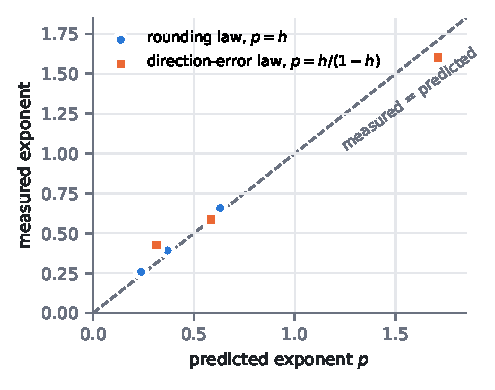
\includegraphics[width=0.78\columnwidth]{figures/fig1_precision_laws.pdf}
\caption{Measured scaling exponent of the noise floor against the prediction, for rounding (circles, three values of
$h$) and for a direction error (squares).}
\label{fig:laws}
\end{figure}

\section{The orbit obstruction and the cost law}
In an exactly skew toy the cross direction is the same at every point, and covariant Lyapunov vectors [6] computed
along a kicked stagger trajectory recover $\lambda_x$ (0.406 vs 0.405). EqR is not skew (Sec.~2). With feedback as
weak as $10^{-3}$ from the decision into the churn, the same pipeline loses the signal and calls a rough toy
filamentary (Fig.~\ref{fig:orbit}): the cross direction now depends on the orbit's own future, which a kicked
pseudo-orbit does not follow. Genuine orbits of $\sim$160 steps, found by bisection [8] at 80 digits without any
kick, restore it (9/9 verdicts correct, $\lambda_x$ within 25\% in 8/9).

\begin{figure}[t]\centering
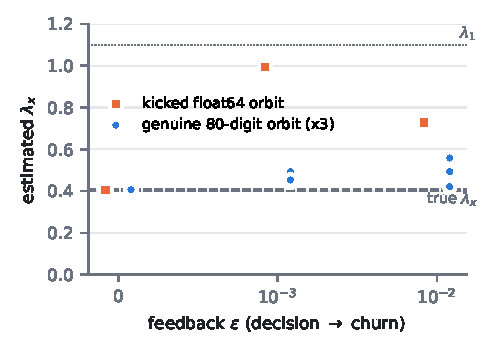
\includegraphics[width=0.78\columnwidth]{figures/fig2_orbit_obstruction.pdf}
\caption{Estimated $\lambda_x$ for a rough toy with feedback $\epsilon$, from kicked float64 orbits (squares) and from
genuine 80-digit orbits (circles, three each).}
\label{fig:orbit}
\end{figure}

Together: a one-decade probe window needs $c\leq0.01^{(1-h)/h}$, a genuine orbit of length
$L\approx L_{\rm warm}+\ln(1/c)/g$ on the chaotic set ($g$: spectral gap above $\lambda_x$), and $\sim L\lambda_1/\ln10$
digits to hold it (toy check: 76 predicted, 80 used). For EqR puzzle 80 ($\lambda_1=2.34$; $h\approx0.105$ if the
boundary is skew-rough) and the measured gaps of 0.05--0.1, this means a genuine orbit of 450--850 loops in 460--860
digits: decidable in principle, out of reach in practice. In float64 no EqR puzzle is decidable: where
stagger-and-step can hold an orbit ($\kappa\leq0.25$) the usable window is below a decade, and where it would open
the orbit cannot be held.

\section{Smaller models?}
The cost does not grow with the size of the latent, so a small trained reasoner might be decidable. Three looped
models trained on $4\times4$ Sudoku (a one-layer residual update with 32 or 64 dimensions; the same with several valid
answers; a miniature EqR with 16 tokens and inner cycles, 94--95\% accurate) never showed transient chaos: easy
puzzles contract ($\lambda_1<0$), and the hardest either settle without an exponential tail or keep oscillating
($\lambda_1\approx0$). In this family, transient chaos appears to need scale.

\section{Limitations}
The degeneracy is an argument with numerical support, not a theorem. The laws are verified on toys of 2--30
dimensions. The EqR price assumes a skew-rough boundary ($h=\kappa/\lambda_1$). One model and one task. Scripts,
pre-registrations (with every amendment and bug fix) and raw outputs exist for every number.

\small
\noindent\textbf{Acknowledgments.} Claude (Anthropic) collaborated on this work as an assistant. All decisions and
claims, and the responsibility for them, rest solely with the author.

\footnotesize
\begin{thebibliography}{9}\setlength{\itemsep}{0pt}
\bibitem{lai26} J.~Lai, A.~Bao, J.~Quinn, W.~Gilpin, \emph{Fractal basins trap latent reasoning}, arXiv:2609.04963 (2026).
\bibitem{bl20} T.~B\'odai, V.~Lucarini, \emph{Rough basin boundaries in high dimension: can we classify them experimentally?}, arXiv:2001.08871 (2020).
\bibitem{kg85} H.~Kantz, P.~Grassberger, Physica D \textbf{17}, 75 (1985).
\bibitem{lt11} Y.-C.~Lai, T.~T\'el, \emph{Transient Chaos}, Springer (2011).
\bibitem{sny01} D.~Sweet, H.~E.~Nusse, J.~A.~Yorke, Phys.\ Rev.\ Lett.\ \textbf{86}, 2261 (2001).
\bibitem{g07} F.~Ginelli \emph{et al.}, Phys.\ Rev.\ Lett.\ \textbf{99}, 130601 (2007).
\bibitem{e26} Euvel, \emph{Escape rate, Lyapunov exponent and the uncertainty exponent of a latent-reasoning model}, \url{https://github.com/euvel/eqr-transient-chaos} (2026).
\bibitem{ny89} H.~E.~Nusse, J.~A.~Yorke, Physica D \textbf{36}, 137 (1989).
\bibitem{g83} C.~Grebogi, S.~W.~McDonald, E.~Ott, J.~A.~Yorke, Phys.\ Lett.\ A \textbf{99}, 415 (1983).
\end{thebibliography}
\end{document}
